\chapter{Introduction}

% Background

How do submarine operators detect the presence of vessels in the waters around them? One of the primary technologies used for this is SOund Navigation And Ranging (sonar), which uses the propagation of sound waves in water to analyse the presence, location, and nature of underwater objects \cite{niu_advances_2023}. Sonar works analogously to how audio recording works in air: sound is carried through the water medium as longitudinal waves with a certain frequency and energy, and this pressure is picked up by a recording device called a hydrophone. These hydrophones convert the mechanical energy of the wave into an electrical signal, which can then be analysed using a variety of methods in the field of \acrfull{dsp} \cite{waite_sonar_2002, domingos_survey_2022}.

Classifying an object based on its sonar signature, a task known as underwater acoustic classification or \acrfull{uatr}, is a difficult job. This process is traditionally split into two stages: feature extraction and classification. Feature extraction focuses on identifying and isolating key attributes from raw sonar signals, while classification involves applying various models to categorise the input signals based on these extracted features (see Figure \ref{fig:luo-flowchart}). Currently, both these tasks are being undertaken by teams of highly-trained sonar technicians around the world \cite{aslam_underwater_2024}. These teams use large databases of patterns and signals collected from known objects over the years to compare and classify a new incoming signal \cite{niu_advances_2023}. It is a slow and cumbersome task which at present relies on traditional rule-based learning techniques \cite{neupane_review_2020}.  However, with recent advancements in artificial intelligence, researchers aim to automate \acrshort{uatr}, making it faster and potentially more accurate \cite{aslam_underwater_2024, neupane_review_2020}. Improving this automation of \acrshort{uatr} is the primary focus of this thesis.

\begin{figure}[htbp]
\centering 
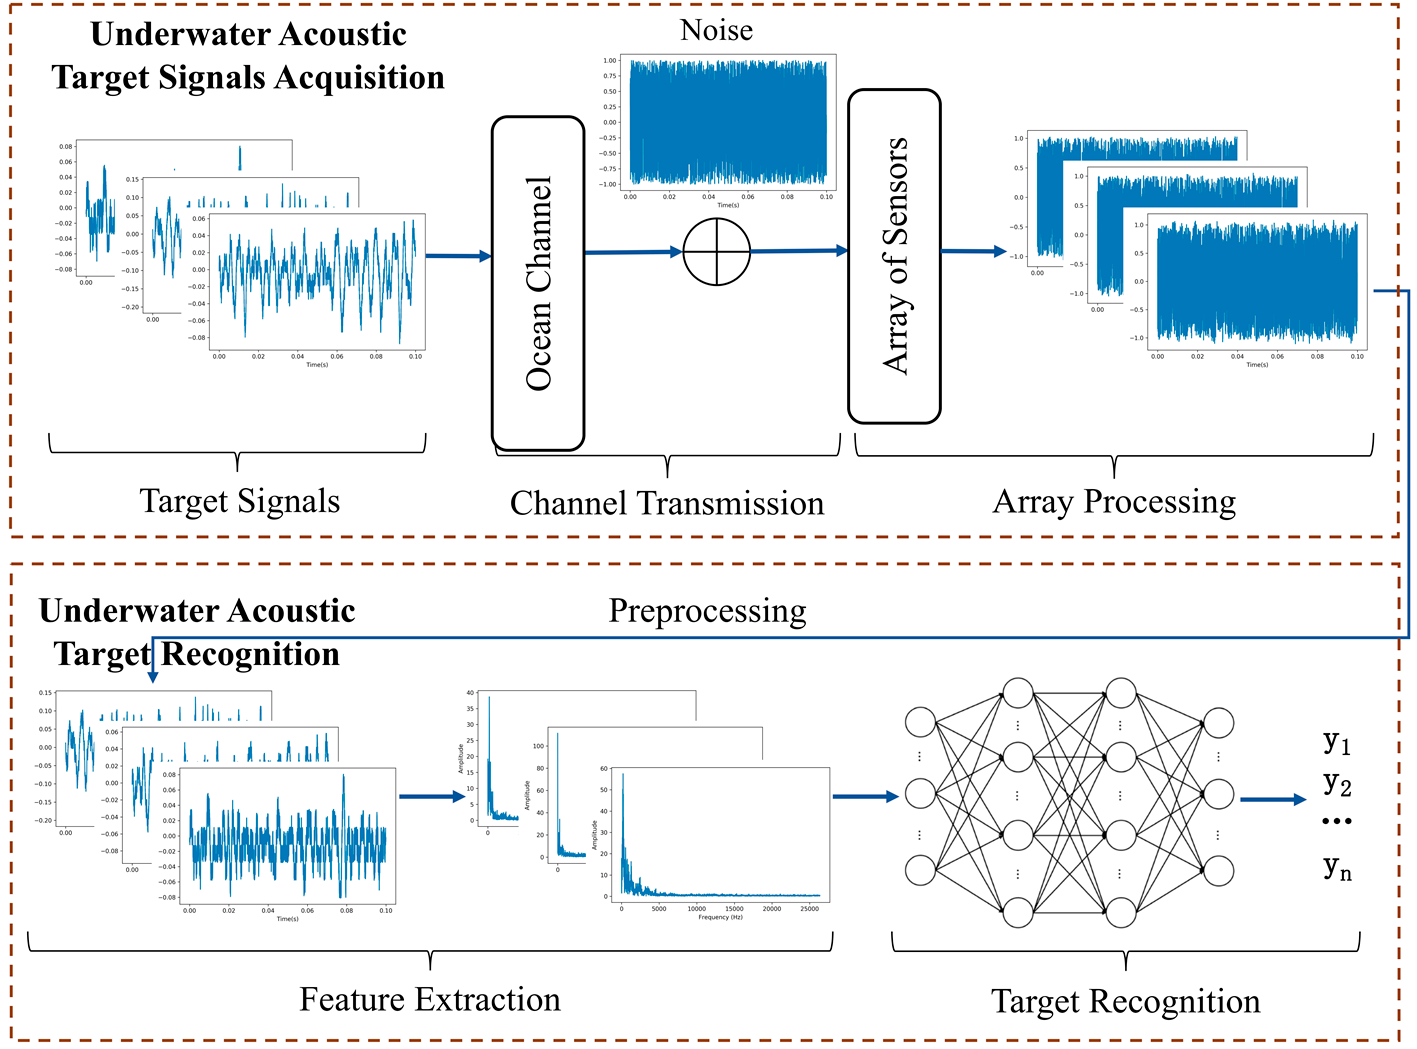
\includegraphics[width=0.8\textwidth]{img/ch1/flowchart.png} 
\caption{Flow chart of underwater acoustic signal acquisition and target recognition, obtained from \cite[Fig.~1]{luo_survey_2023}} 
\label{fig:luo-flowchart} 
\end{figure}

\section{Problem statement}

The underwater acoustic environment is inherently noisy and unpredictable. Factors such as signal reflection, refraction, and attenuation, as well as the variety of noise sources underwater, including marine life, vessel traffic, and environmental disturbances, introduce significant distortion to recorded signals. These factors create highly variable and noisy recordings, complicating the extraction of meaningful features needed for accurate target classification. Preprocessing techniques, such as denoising and detrending, play an important part in enhancing the quality of sonar signals by reducing noise and highlighting relevant characteristics which are important for downstream classification tasks.

Once the quality of model inputs is improved through preprocessing, the next step in \acrshort{uatr} is feature extraction. Traditional methods rooted in \acrshort{dsp} have canonically been the go-to methods for capturing meaningful characteristics of acoustic signals. These approaches have provided a reliable foundation for \acrshort{uatr} systems for decades. However, with the advent of deep learning, there is now an opportunity to complement these well-established approaches by exploring automated feature extraction. Deep learning models, particularly those designed for unsupervised learning or transfer learning, can potentially uncover latent, high-dimensional features which could enhance the accuracy and adaptability of UATR systems.

Despite this potential, there is limited research systematically exploring the effect of traditional preprocessing and feature extraction methods with modern deep learning-based approaches in the context of UATR. The unique challenges of the underwater environment, such as limited labelled data and the inherent variability of sonar signals, calls for a tailored investigation into the effectiveness of these methods.

This thesis addresses this knowledge gap by investigating advanced preprocessing techniques such as denoising and detrending and leveraging deep learning to explore automated feature extraction. Through a comprehensive evaluation of these methods, this work aims to build upon and extend existing work in the field to improve the accuracy and robustness of UATR systems.

\section{Proposed solution}

This thesis aims to improve the accuracy of UATR models by enhancing feature representations, focusing on two main areas: preprocessing techniques, to refine raw input signals, and deep feature extraction, to uncover latent, meaningful features automatically. Keeping a constant benchmark classifier (CNN-LSTM), we systematically experiment with different preprocessing and feature extraction techniques to evaluate their impact on classification performance. This approach enables us to isolate the effects of feature improvements from those of classification model changes.

In the area of preprocessing techniques, we investigate various normalisation, detrending and denoising strategies. Firstly, we aim to quantify the effects of channel-based normalisation and global normalisation on spectrogram inputs into deep learning models. Then, we explore the use of the $\ell_1$ detrending algorithm, which removes long-term, low-frequency trends in the acoustic signal, helping to emphasise short-term variations that are more likely to capture unique target characteristics. Additionally, experiments in denoising are undertaken to evaluate the effectiveness of noise reduction frameworks, particularly the Noise2Noise methodology. Noise2Noise enables denoising without needing access to clean reference signals, making it suitable for the underwater environment where obtaining clean ground truth is impossible.

In the area of deep feature extraction, two main approaches are tested. The first approach leverages autoencoders to automatically generate a compact latent space representation from input spectrograms. Unlike traditional, manually crafted feature extraction methods, which rely heavily on domain-specific knowledge and human intervention, autoencoders aim to learn informative features directly from raw data. This approach bypasses the need for extensive domain expertise and allows us to potentially uncover latent patterns that could be missed by conventional methods. The second approach involves transfer learning. First, a pretrained transformer-based model, the Audio Spectrogram Transformer, is fine-tuned on the labelled DeepShip dataset to evaluate improvements in classification accuracy. Following this, we experiment with training an autoencoder on an unlabelled acoustic dataset and using the learned features as input to the CNN-LSTM classifier tested on DeepShip. Together, these strategies in deep feature extraction allow the model to benefit from both supervised fine-tuning and unsupervised representation learning.

By applying these methods with a consistent CNN-LSTM classifier, this thesis assesses the contribution of each feature extraction technique, allowing for a precise evaluation of their impact on UATR performance.

\section{Key contributions}

\textit{TO DO.}

% \section{Motivation}

% How do submarine operators detect the presence of vessels in the waters around them? One of the primary technologies used in naval navigation is SOund Navigation And Ranging (sonar), which uses the propagation of sound waves in water as a tool for communication, object detection, and source localisation, among other tasks \cite{niu_advances_2023}.

% Sonar works analogously to how audio recording works in air. Sound is carried through the water medium as longitudinal waves with a certain frequency and energy, and this pressure is picked up by a recording device called a hydrophone. These hydrophones convert the mechanical energy of the wave into an electrical signal, which can then be analysed using a variety of methods in the field of digital signal processing \cite{waite_sonar_2002, domingos_survey_2022}.

% Classifying an object based on its sound signature, a task known as underwater acoustic classification or \acrfull{uatr}, is a difficult job. There are two main stages involved: a) feature extraction, which involves selecting and computing the most useful properties of the incoming sonar signal, and b) target classification, which uses the aforementioned features to try and classify the signal's source (Figure \ref{fig:luo-flowchart}). Currently, these procedures are being undertaken by teams of highly-trained sonar technicians around the world \cite{aslam_underwater_2024}. These teams use large databases of patterns and signals collected over the years from known objects to compare and classify a new incoming signal \cite{niu_advances_2023}. It is a slow and cumbersome task which at present relies on traditional rule-based learning techniques \cite{neupane_review_2020}. 

% \begin{figure}[htbp]
%     \centering
%     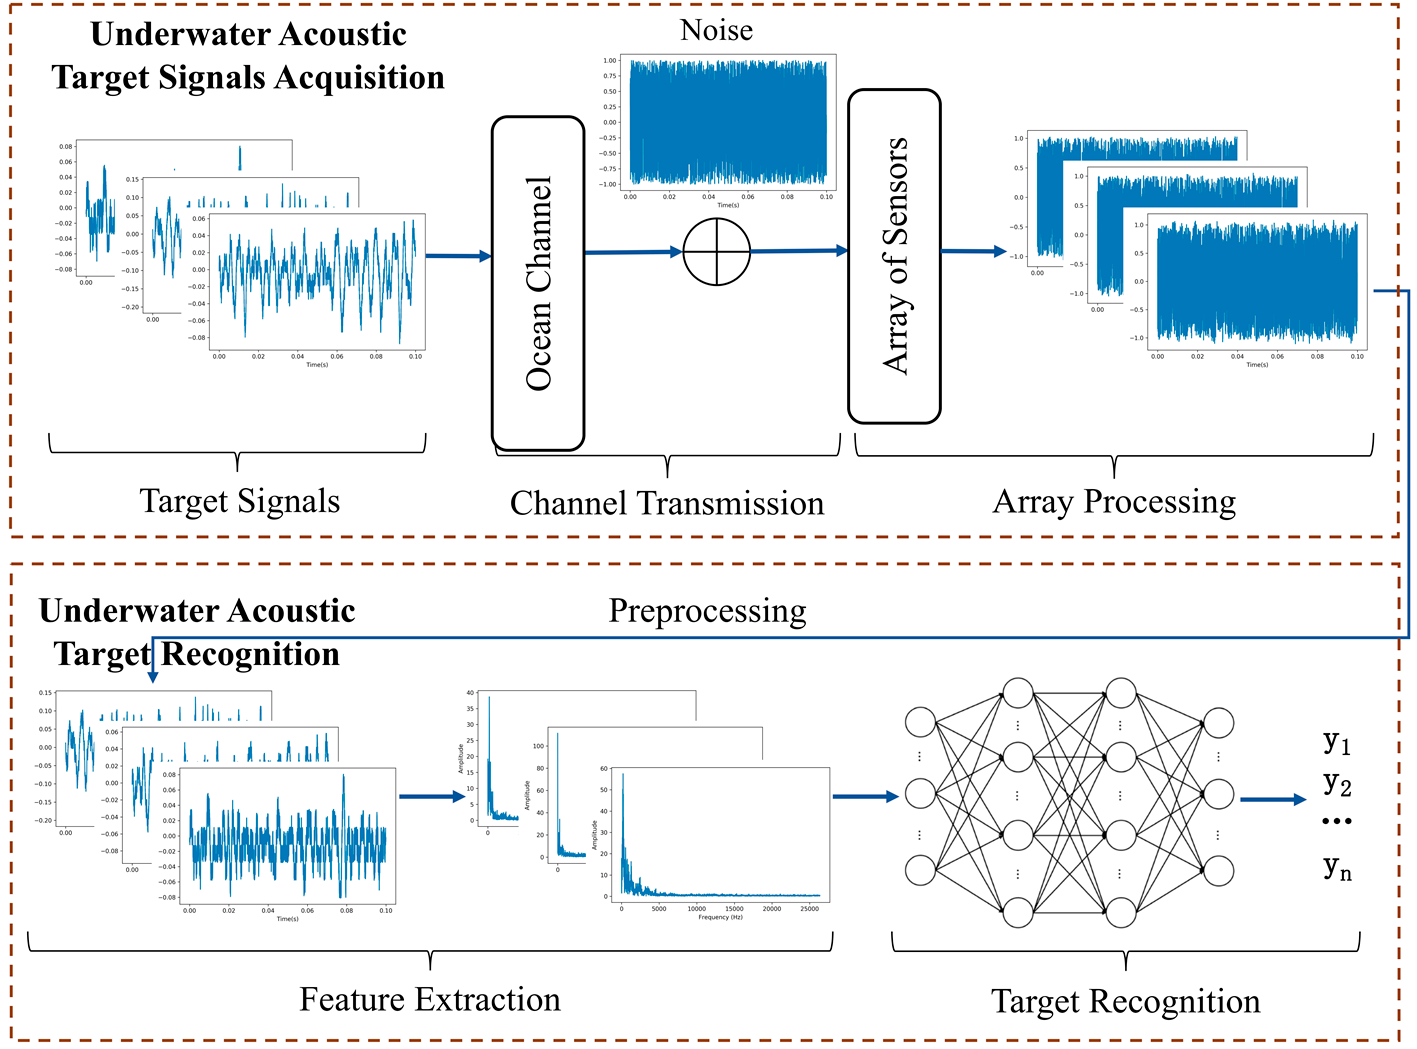
\includegraphics[width=0.8\textwidth]{img/ch1/flowchart.png}
%     \caption{Flow chart of underwater acoustic signal acquisition and target recognition, obtained from \cite[Fig.~1]{luo_survey_2023}}
%     \label{fig:luo-flowchart}
% \end{figure}

% However, with recent advancements in \acrfull{ai}, researchers are looking to optimise this \acrshort{uatr} process by employing \acrfull{ml} techniques to automatically classify a vessel given its passive sonar signal output \cite{neupane_review_2020}. A real-time classification system deployed underwater would save sonar operators thousands of hours in manual processing and classification time, as well as be able to provide live classifications to the crew on-board without having to rely on land-based operators \cite{aslam_underwater_2024}. This would reduce rates of false negatives, which, in a national security setting such as the detection of foreign vessels in sovereign waters, can be extremely costly.

% \section{Problem statement}

% In many existing \acrlong{ml}-based classification systems, raw sonar signals are processed using traditional digital signal processing techniques to convert them into more interpretable features. For example, one commonly used method is the \acrfull{stft}, which transforms the input signal into a time-frequency representation, resulting in a spectrogram. This spectrogram is then passed into various classification models, ranging from conventional algorithms like \acrfull{knn} and \acrfull{svm} to more advanced deep learning architectures such as \acrfull{cnn}, \acrfull{rnn}, and \acrfull{lstm}.

% As Bengio et al. emphasise, ``the performance of machine learning methods is heavily dependent on the choice of data representation (or features) on which they are applied'' \cite{bengio_representation_2013}. This brings us to a fundamental challenge: how can we ensure that a spectrogram -- or any other feature we extract -- is truly the \textit{optimal} representation for accurate classification?

% Indeed, the ultimate goal in feature engineering is to identify the most informative and distinguishing features that can enhance the classifier’s ability to accurately categorise input signals. My role in this project involves addressing this challenge by exploring representation learning techniques to automate the feature extraction process. By leveraging self-supervised and unsupervised learning methods, I aim to automatically uncover latent features within the raw data, without relying on predefined feature sets. This approach seeks to extend beyond traditional feature engineering, allowing for deeper and more meaningful representations, ultimately leading to improved classification performance.

\section{Outline}

The structure of this thesis is as follows:

\paragraph{Chapter 2: Background and Literature Review} This chapter provides essential theoretical background for readers, covering key aspects of underwater acoustic signal propagation, such as noise sources and their impact on signal quality, which are relevant for the denoising work explored later. The chapter also offers an introduction to artificial intelligence and concludes with a comprehensive literature review, summarising over 50 foundational and recent high-impact studies within the field.

\paragraph{Chapter 3: Establishing a Benchmark Performance} Here, we establish the CNN-LSTM architecture as the benchmark classifier model for our experiments, detailing its inputs, structure, configuration, and baseline performance metrics. This consistent architecture serves as a point of reference for evaluating all subsequent feature-related modifications.

\paragraph{Chapter 4: Experiments in Preprocessing Techniques} This chapter delves into various preprocessing techniques to enhance raw input data quality, focusing on methods such as normalisation, detrending and denoising. We assess the impact of these techniques on the classification performance of the benchmark model.

\paragraph{Chapter 5: Experiments with Deep Feature Extraction} Building on preprocessing improvements, this chapter explores advanced feature extraction approaches, including the application of autoencoders and transfer learning. We investigate how these methods affect model accuracy, offering insight into the effectiveness of learned representations for underwater acoustic target recognition.